\chapter{THỬ NGHIỆM VÀ KẾT QUẢ}

\section{Thiết lập môi trường thử nghiệm}
Mọi thí nghiệm được thực hiện trên cùng một môi trường phần cứng, cố định hạt giống ngẫu nhiên \texttt{random\_state = 42} để đảm bảo tính tái lập 100\%. Dữ liệu được đọc trực tiếp từ tệp \texttt{data/raw/hotel\_bookings.csv}.

\section{Cấu hình dữ liệu train/test}
\begin{itemize}
    \item Tổng số mẫu: 119,390 dòng.
    \item Tập huấn luyện (Train Set -- 80\%): 95,512 mẫu (60,133 mẫu không hủy, 35,379 mẫu hủy).
    \item Tập kiểm thử độc lập (Test Set -- 20\%): 23,878 mẫu (15,033 mẫu không hủy, 8,845 mẫu hủy).
    \item Tỷ lệ hủy phòng tại cả hai tập: $37.04\%$.
\end{itemize}

\section{Thiết lập Baseline (EXP01)}
Mô hình cơ sở \texttt{DummyClassifier(strategy='most\_frequent')} dự đoán toàn bộ 23,878 mẫu kiểm thử là Lớp 0 (Không hủy).
\begin{itemize}
    \item \textbf{Accuracy:} $62.96\%$ (đúng bằng tỷ lệ mẫu Lớp 0 trong tập test).
    \item \textbf{Precision (Lớp 1):} $0.00\%$.
    \item \textbf{Recall (Lớp 1):} $0.00\%$ (bỏ sót toàn bộ 8,845 đơn đặt phòng bị hủy).
    \item \textbf{F1-Score (Lớp 1):} $0.00\%$.
    \item \textbf{ROC-AUC:} $0.5000$.
\end{itemize}

\section{Kết quả Pipeline A (Tiền xử lý cơ bản)}
Trên Pipeline A (sử dụng đặc trưng gốc, mã hóa One-Hot toàn bộ và chuẩn hóa tiêu chuẩn):
\begin{itemize}
    \item \textbf{EXP02 (KNN, k=7):} Đạt Accuracy $82.63\%$, Precision $77.88\%$, Recall $74.18\%$, F1-Score $75.98\%$ và ROC-AUC $0.8949$.
    \item \textbf{EXP03 (Decision Tree, max\_depth=10):} Đạt Accuracy $84.42\%$, Precision $82.16\%$, Recall $74.02\%$, F1-Score $77.88\%$ và ROC-AUC $0.9230$.
\end{itemize}

\section{Kết quả Pipeline B (Cải tiến với Feature Engineering)}
Khi áp dụng các đặc trưng phái sinh (\texttt{total\_nights}, \texttt{total\_guests}, \texttt{room\_type\_changed}, v.v.) và gom nhóm danh mục hiếm:
\begin{itemize}
    \item \textbf{EXP04 (KNN, k=7):} Accuracy tăng lên $82.93\%$, Recall tăng lên $75.48\%$, F1-Score tăng lên $76.61\%$ và ROC-AUC đạt $0.8965$. Pipeline B đã giúp KNN tăng cả 3 chỉ số quan trọng so với Pipeline A.
    \item \textbf{EXP05 (Decision Tree Balanced):} Nhờ trọng số lớp cân bằng, Recall tăng vọt lên \textbf{82.44\%} (phát hiện được 7,292 trên 8,845 ca hủy), F1-Score đạt $79.56\%$.
    \item \textbf{EXP06 (Decision Tree Tuned):} Mô hình cây được tối ưu với độ sâu \texttt{max\_depth=15} và tiêu chí Entropy đạt hiệu năng tổng thể cao nhất: Accuracy \textbf{85.48\%}, F1-Score \textbf{80.12\%} và ROC-AUC \textbf{0.9289}.
\end{itemize}

\section{Bảng so sánh tổng hợp các mô hình}
Bảng \ref{tab:model_comparison} tổng hợp kết quả chạy thực nghiệm từ tệp \texttt{reports/results/model\_test\_comparison.csv}:

\begin{table}[H]
    \centering
    \small
    \caption{Bảng tổng hợp kết quả đánh giá trên tập kiểm thử độc lập (Test Set)}
    \label{tab:model_comparison}
    \begin{tabular}{llccccc}
        \toprule
        \textbf{Mã Thí Nghiệm} & \textbf{Tên Mô Hình} & \textbf{Pipeline} & \textbf{Accuracy} & \textbf{Precision} & \textbf{Recall} & \textbf{F1-Score} \\
        \midrule
        EXP01 & DummyClassifier (Baseline) & Baseline & 0.6296 & 0.0000 & 0.0000 & 0.0000 \\
        EXP02 & KNN ($k=7$) & Pipeline A & 0.8263 & 0.7788 & 0.7418 & 0.7598 \\
        EXP03 & Decision Tree ($d=10$) & Pipeline A & 0.8442 & \textbf{0.8216} & 0.7402 & 0.7788 \\
        EXP04 & KNN ($k=7$) & Pipeline B & 0.8293 & 0.7777 & 0.7548 & 0.7661 \\
        EXP05 & Decision Tree (Balanced) & Pipeline B & 0.8431 & 0.7687 & \textbf{0.8244} & 0.7956 \\
        EXP06 & Decision Tree Tuned & Pipeline B & \textbf{0.8548} & 0.8127 & 0.7901 & \textbf{0.8012} \\
        \bottomrule
    \end{tabular}
\end{table}

\begin{table}[H]
    \centering
    \small
    \caption{Chi tiết ma trận nhầm lẫn của các mô hình trên tập kiểm thử (23,878 mẫu)}
    \label{tab:confusion_matrices_raw}
    \begin{tabular}{lcccc}
        \toprule
        \textbf{Mã Thí Nghiệm} & \textbf{True Negative (TN)} & \textbf{False Positive (FP)} & \textbf{False Negative (FN)} & \textbf{True Positive (TP)} \\
        \midrule
        EXP01: Dummy & 15,033 & 0 & 8,845 & 0 \\
        EXP02: KNN (Pipe A) & 13,169 & 1,864 & 2,284 & 6,561 \\
        EXP03: DT (Pipe A) & 13,611 & 1,422 & 2,298 & 6,547 \\
        EXP04: KNN (Pipe B) & 13,125 & 1,908 & 2,169 & 6,676 \\
        EXP05: DT Balanced (Pipe B) & 12,839 & 2,194 & \textbf{1,553} & \textbf{7,292} \\
        EXP06: DT Tuned (Pipe B) & \textbf{13,422} & 1,611 & 1,857 & 6,988 \\
        \bottomrule
    \end{tabular}
\end{table}

\section{Trực quan hóa đánh giá mô hình}
Hình \ref{fig:model_evaluation} thể hiện đường cong ROC và biểu đồ so sánh các chỉ số giữa 6 mô hình:

\begin{figure}[H]
    \centering
    \begin{subfigure}{0.48\textwidth}
        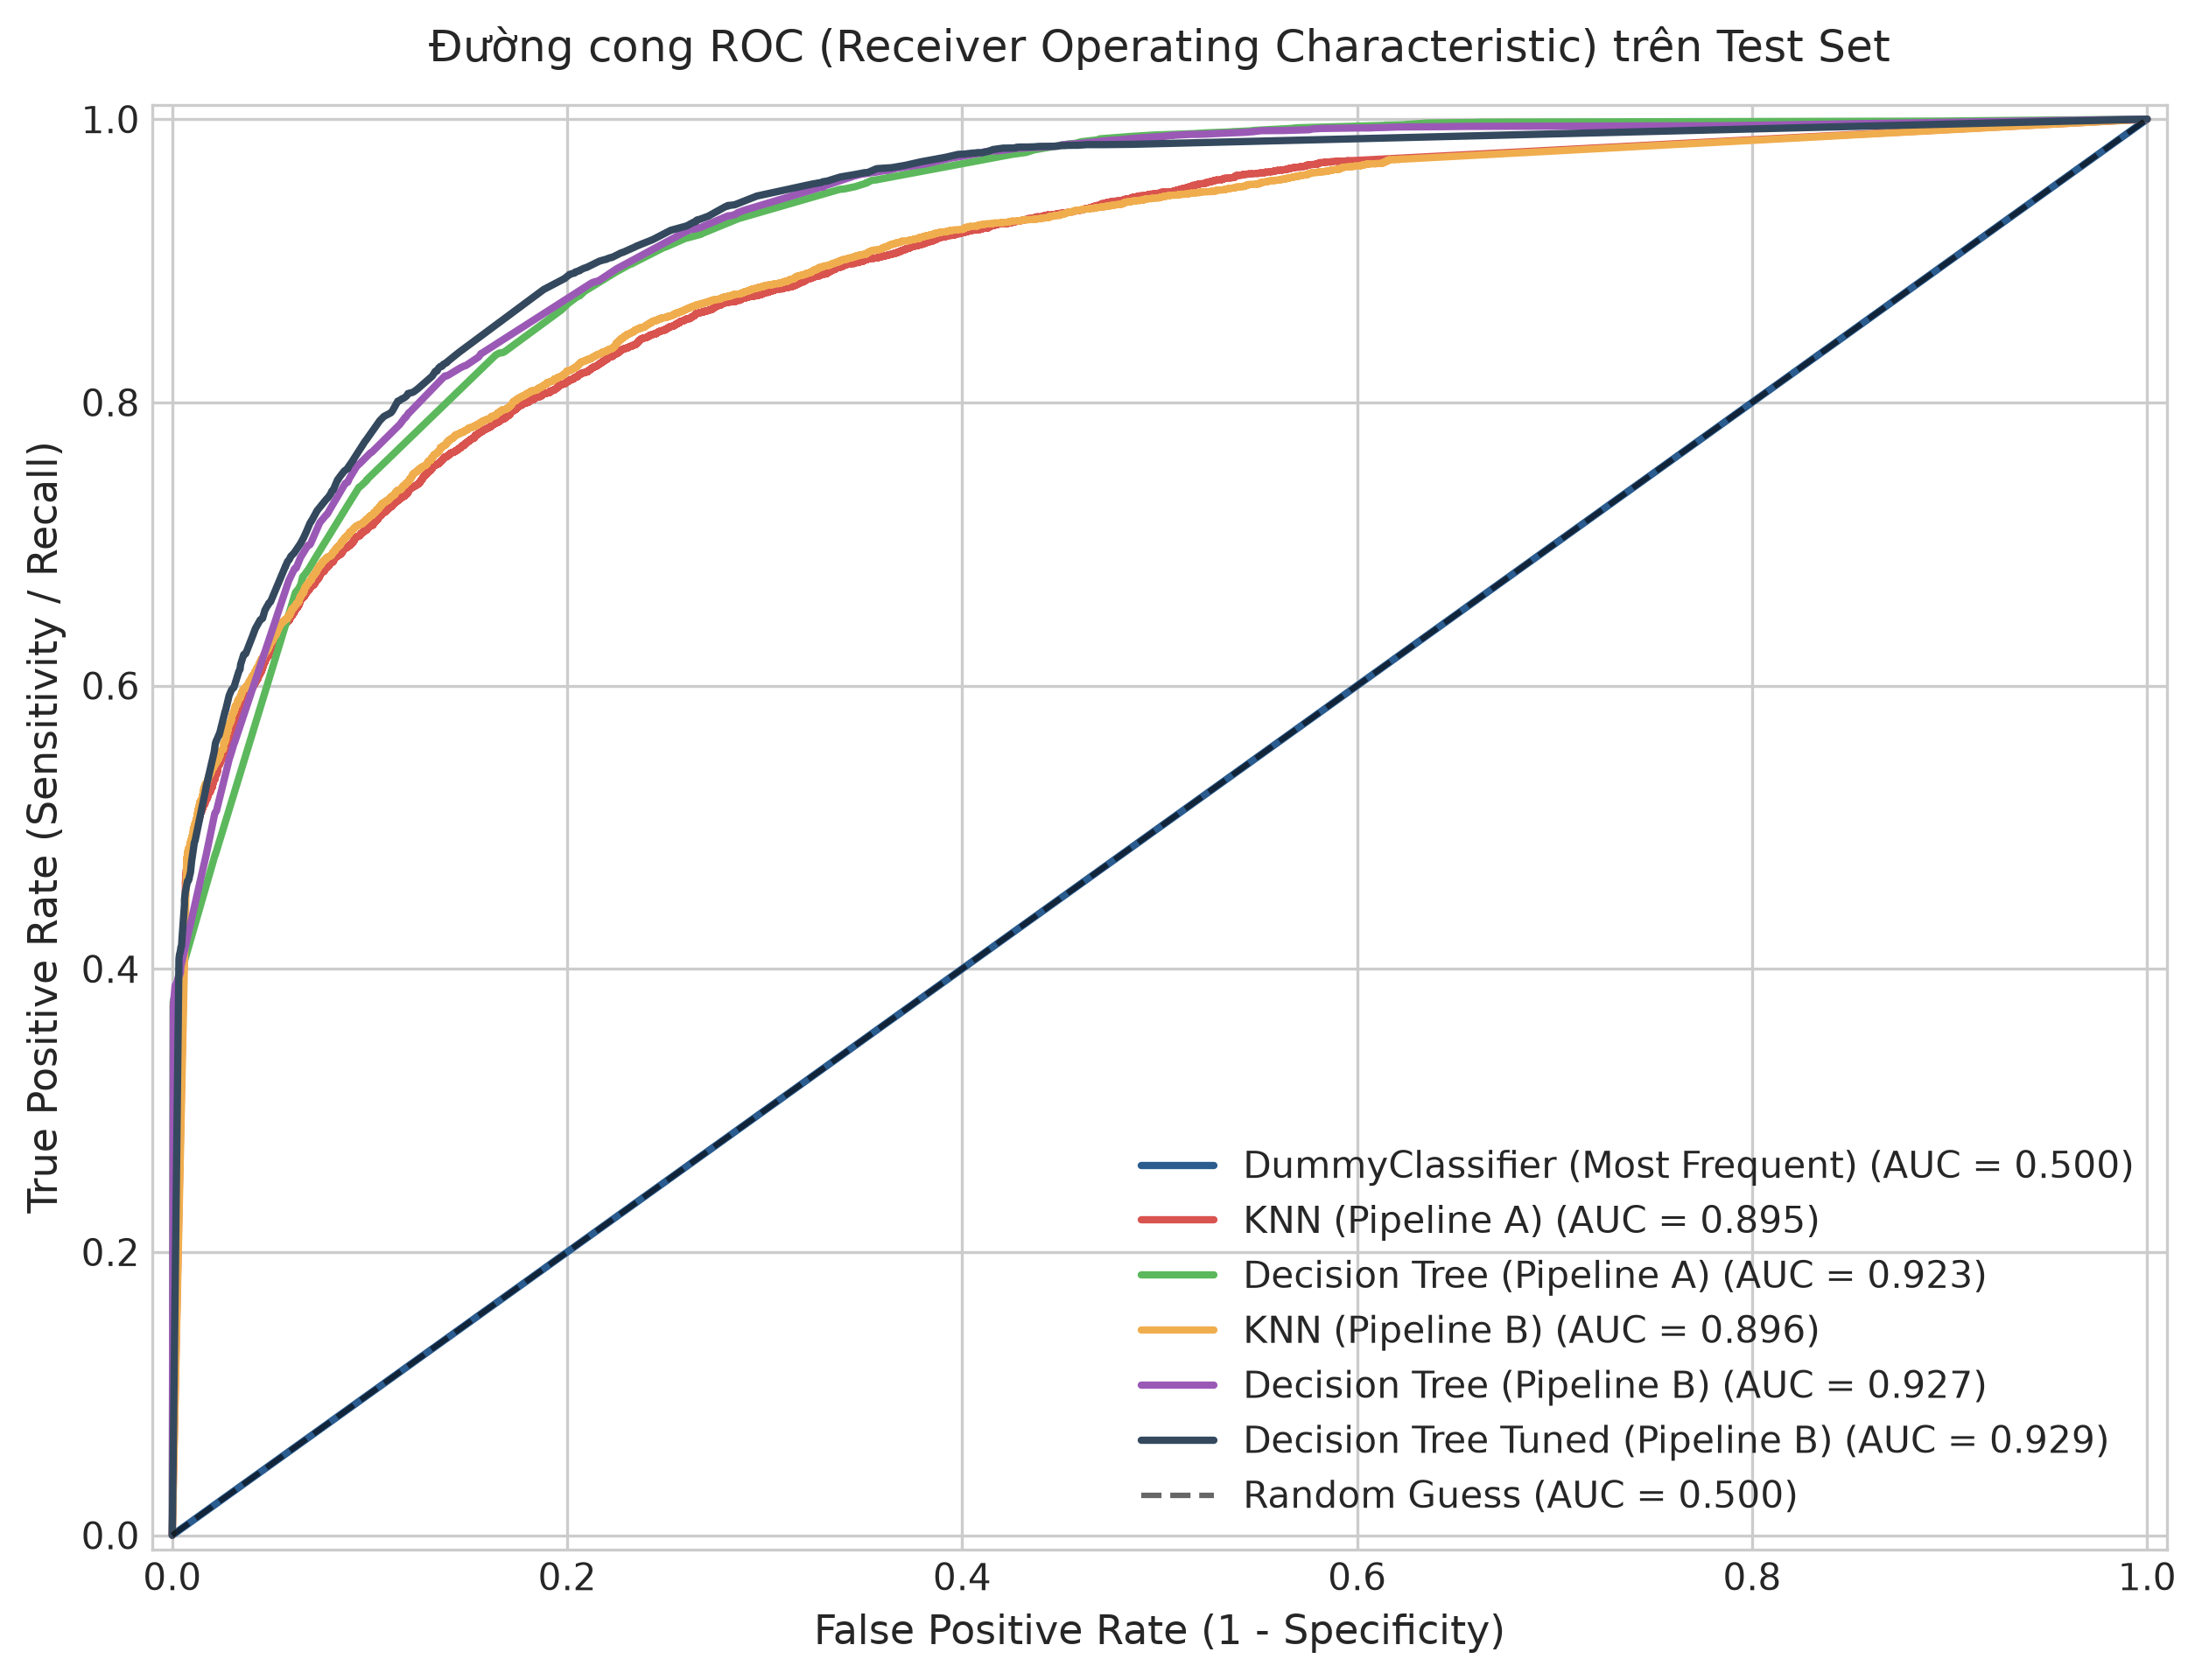
\includegraphics[width=\linewidth]{roc_curves_comparison.png}
        \caption{So sánh đường cong ROC}
    \end{subfigure}
    \begin{subfigure}{0.48\textwidth}
        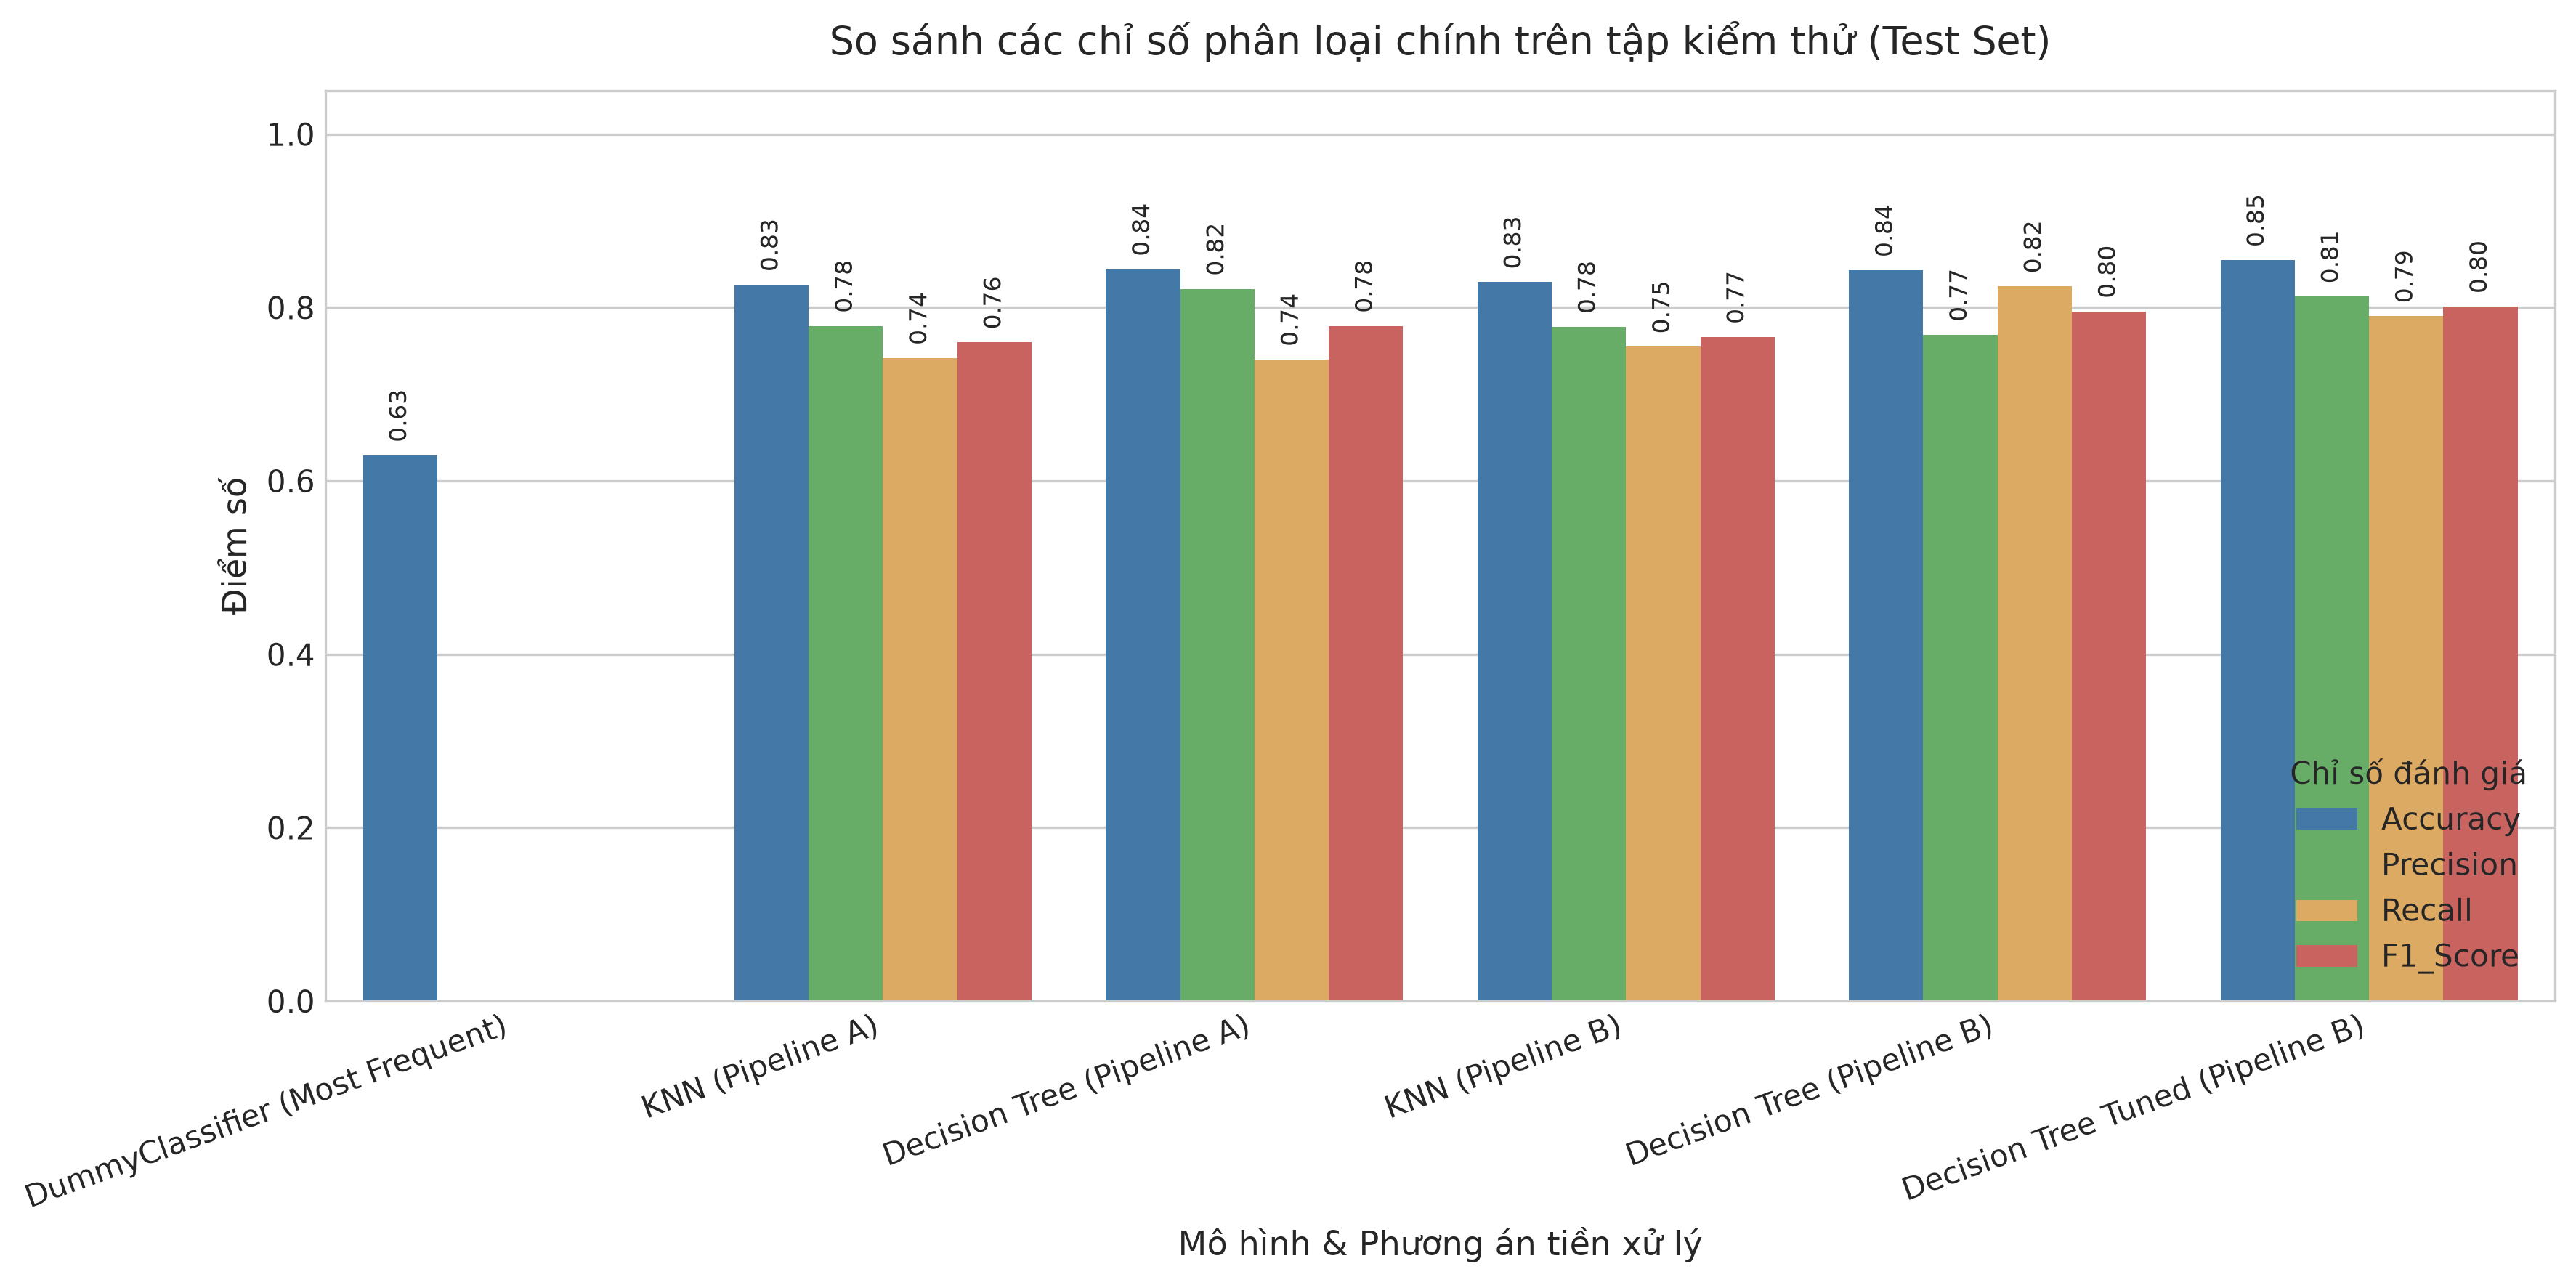
\includegraphics[width=\linewidth]{model_metrics_comparison.png}
        \caption{So sánh các chỉ số phân loại}
    \end{subfigure}
    \caption{Đánh giá trực quan hiệu năng các mô hình trên tập kiểm thử}
    \label{fig:model_evaluation}
\end{figure}

\begin{figure}[H]
    \centering
    \begin{subfigure}{0.48\textwidth}
        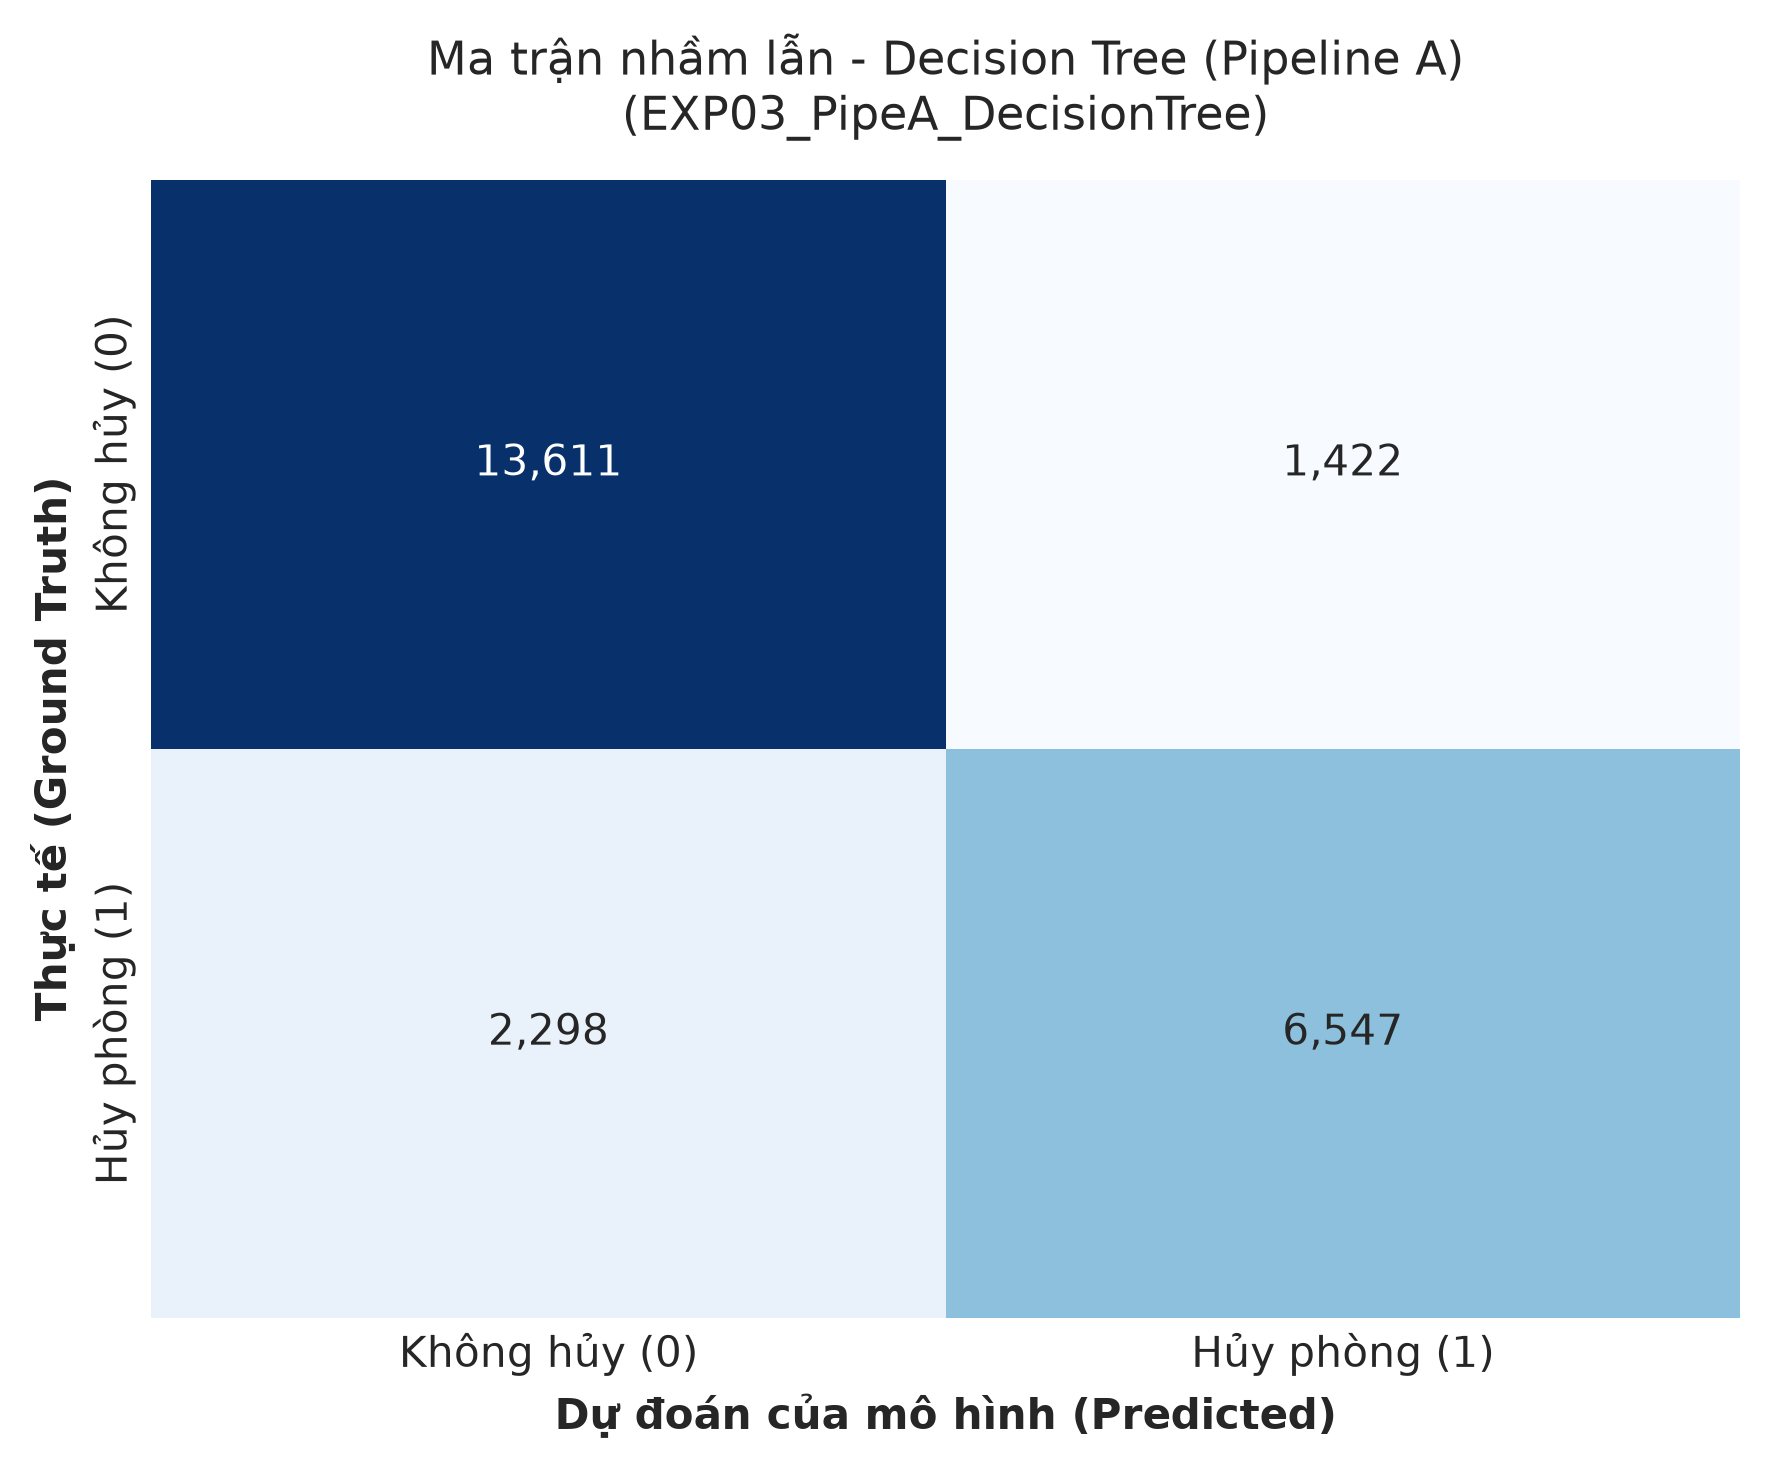
\includegraphics[width=\linewidth]{confusion_matrix_exp03_pipea_decisiontree.png}
        \caption{Ma trận nhầm lẫn EXP03 (DT Pipe A)}
    \end{subfigure}
    \begin{subfigure}{0.48\textwidth}
        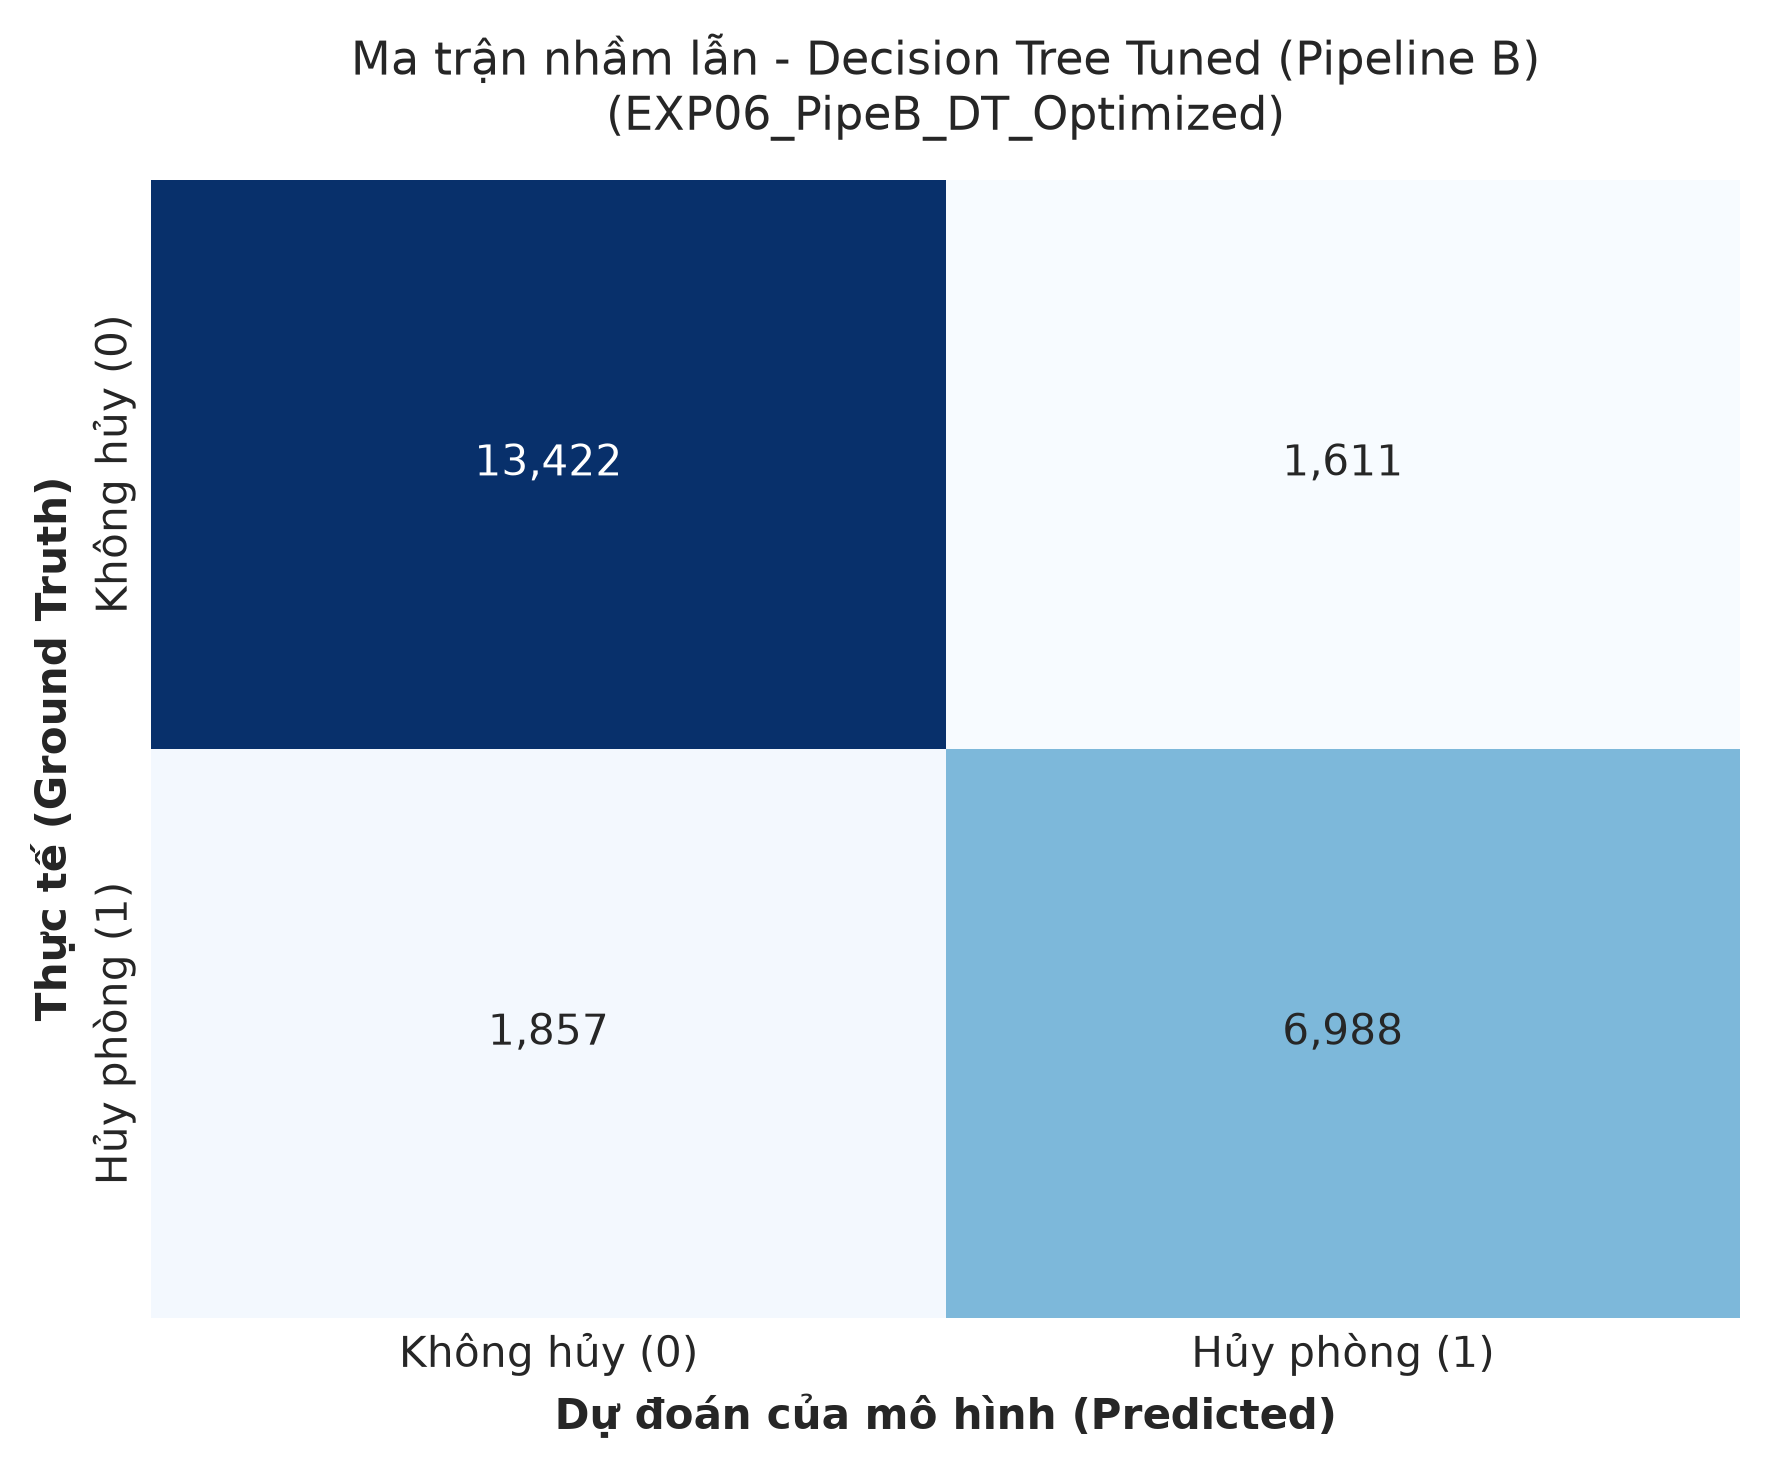
\includegraphics[width=\linewidth]{confusion_matrix_exp06_pipeb_dt_optimized.png}
        \caption{Ma trận nhầm lẫn EXP06 (DT Tuned Pipe B)}
    \end{subfigure}
    \caption{So sánh ma trận nhầm lẫn giữa Decision Tree trên Pipeline A và Pipeline B}
    \label{fig:confusion_matrices}
\end{figure}
